\chapter{Estatísticas e Resultados}

É importante referir uma grande consideração feita na elaboração desta estatísticas
que foi o facto de todos os delay slots serem utilizados uniformemente, ou seja, frequência absoluta uniforme (na prática um delay slot pode ter uma frequência absoluta muito superior a outro).

\begin{figure}[H]
	\begin{center}
		\makebox[\textwidth][c]{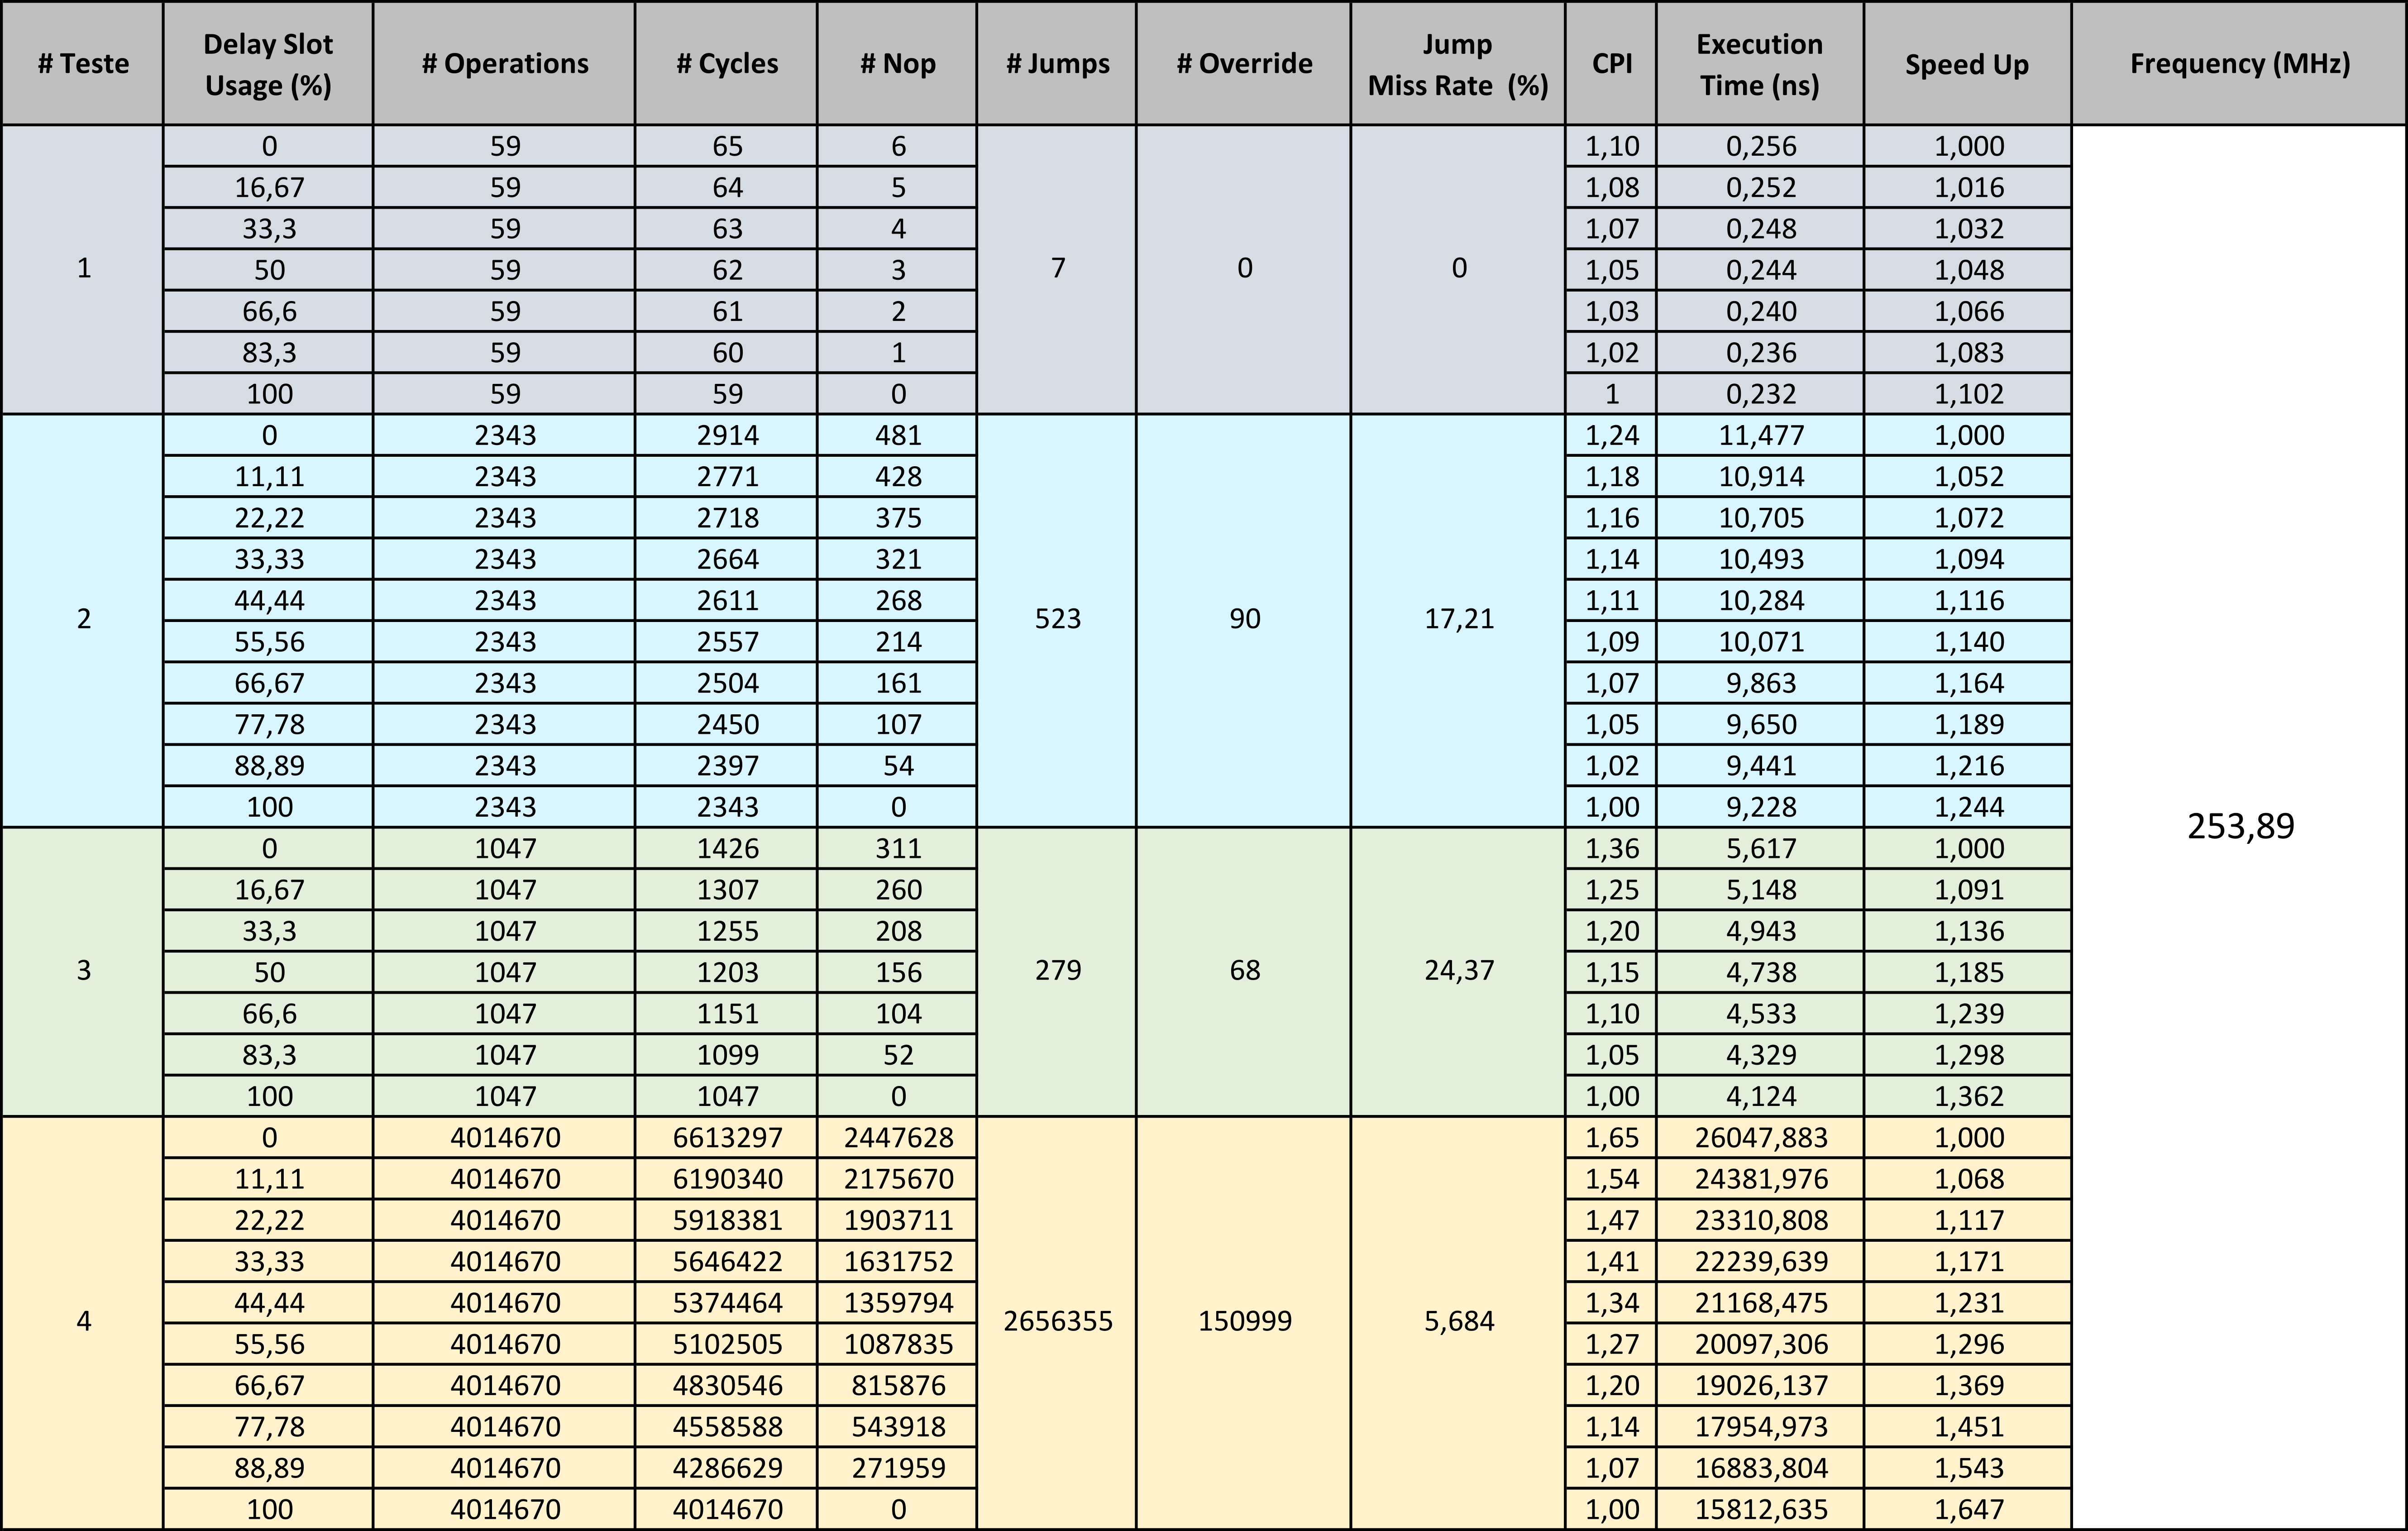
\includegraphics[clip, keepaspectratio=true, scale=1]{./images/tabela.png}}
		\caption{Estatísticas do Pipeline para os Testes realizados.}
		\label{tabela}
	\end{center}
\end{figure}

\begin{figure}[H]
	\begin{center}
		\makebox[\textwidth][c]{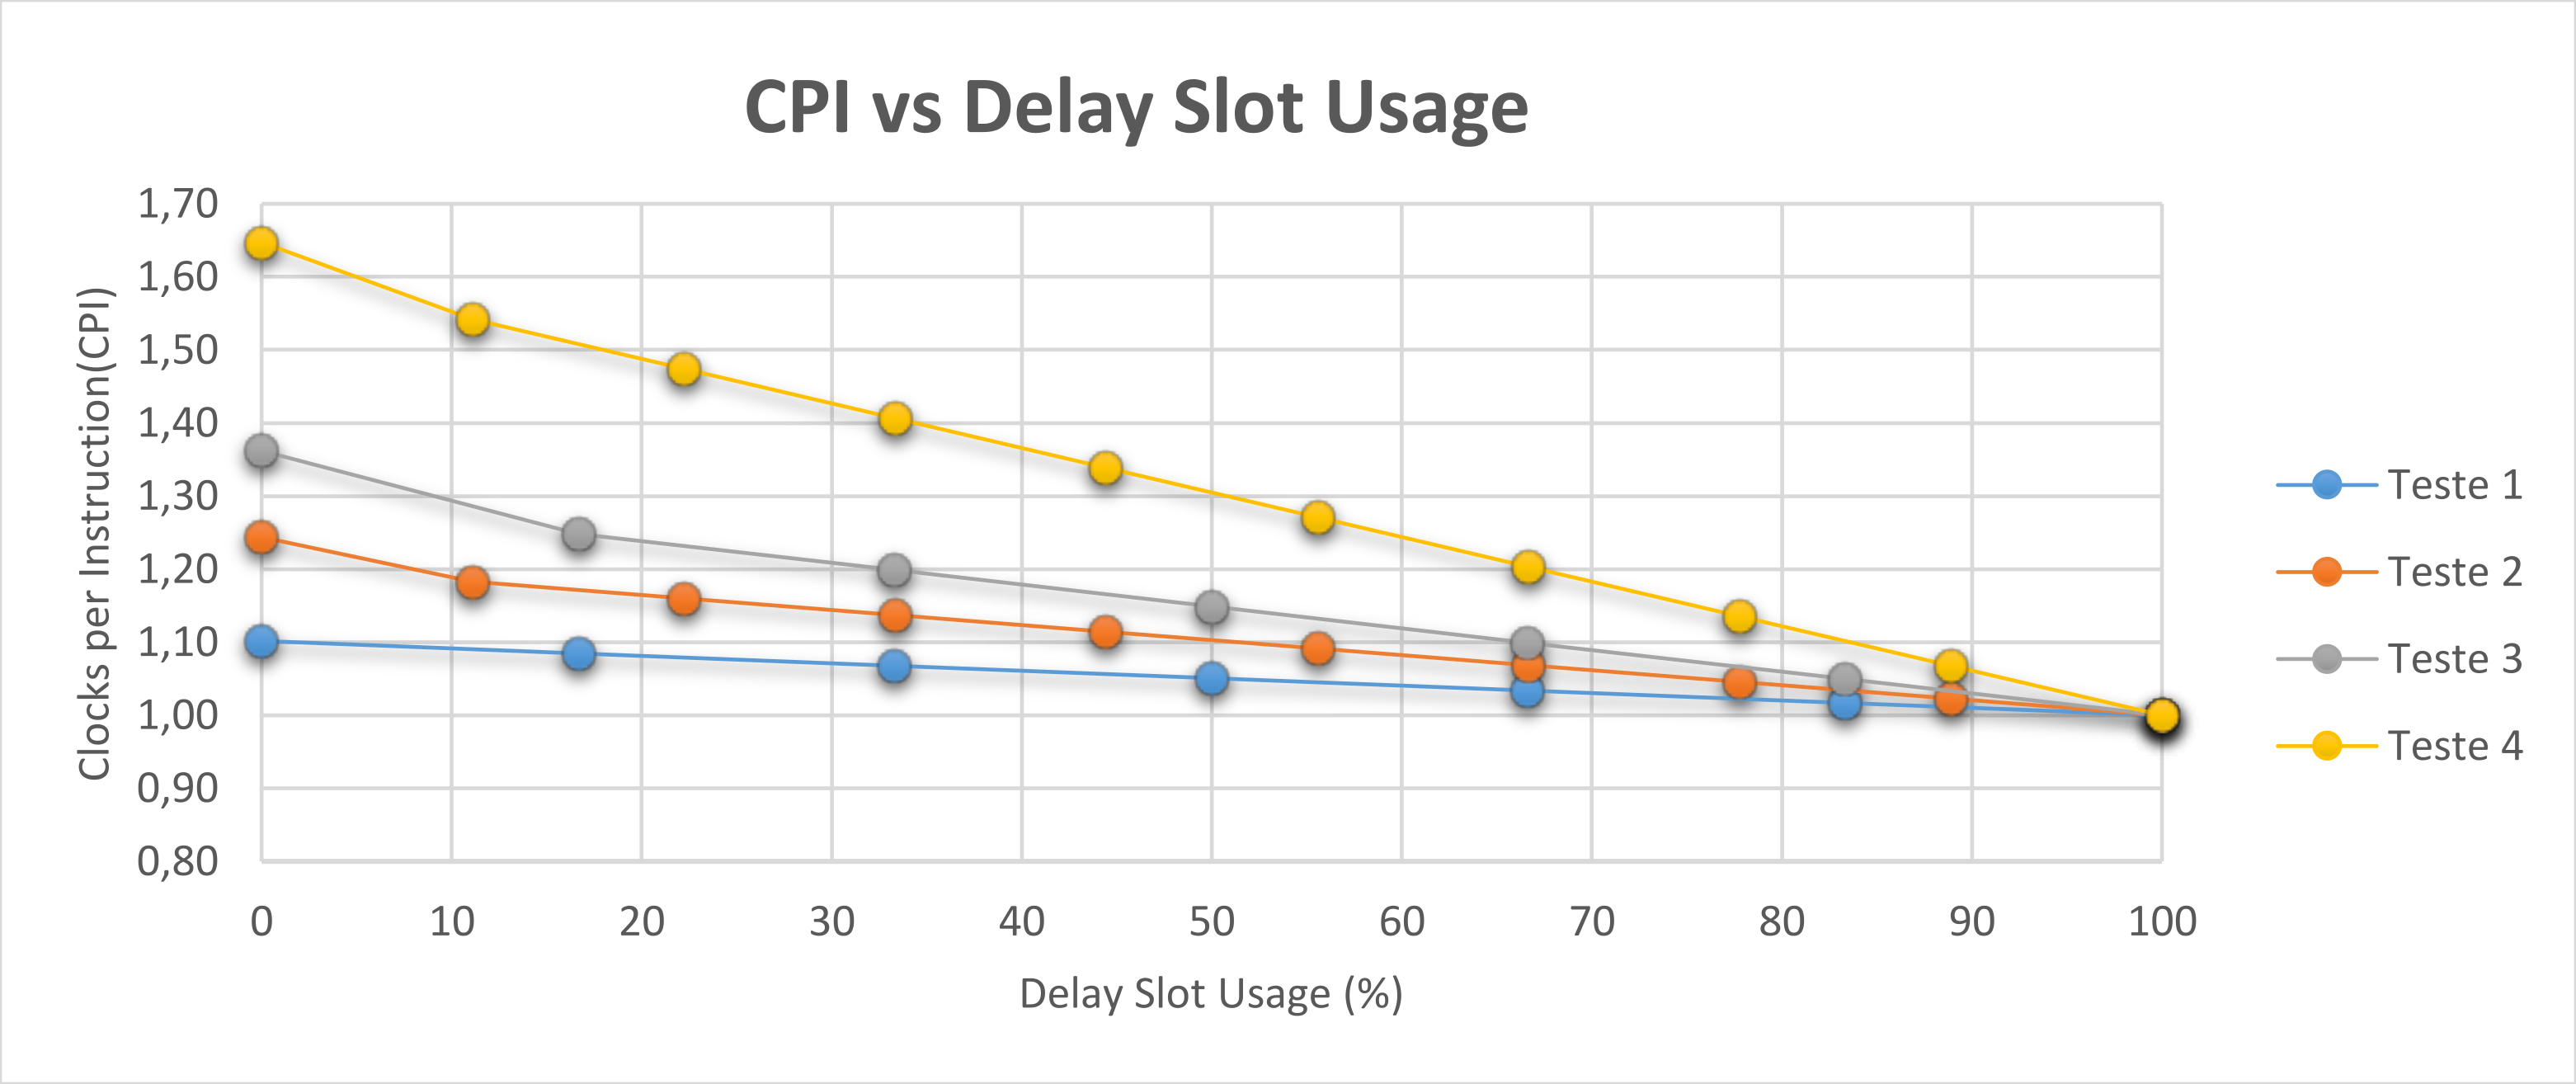
\includegraphics[clip, keepaspectratio=true, scale=1]{./images/cpi.png}}
		\caption{Relação CPI - Utilização do Delay Slot para os Testes 1,2,3 e 4.}
		\label{cpi}
	\end{center}
\end{figure}

\begin{figure}[H]
	\begin{center}
		\makebox[\textwidth][c]{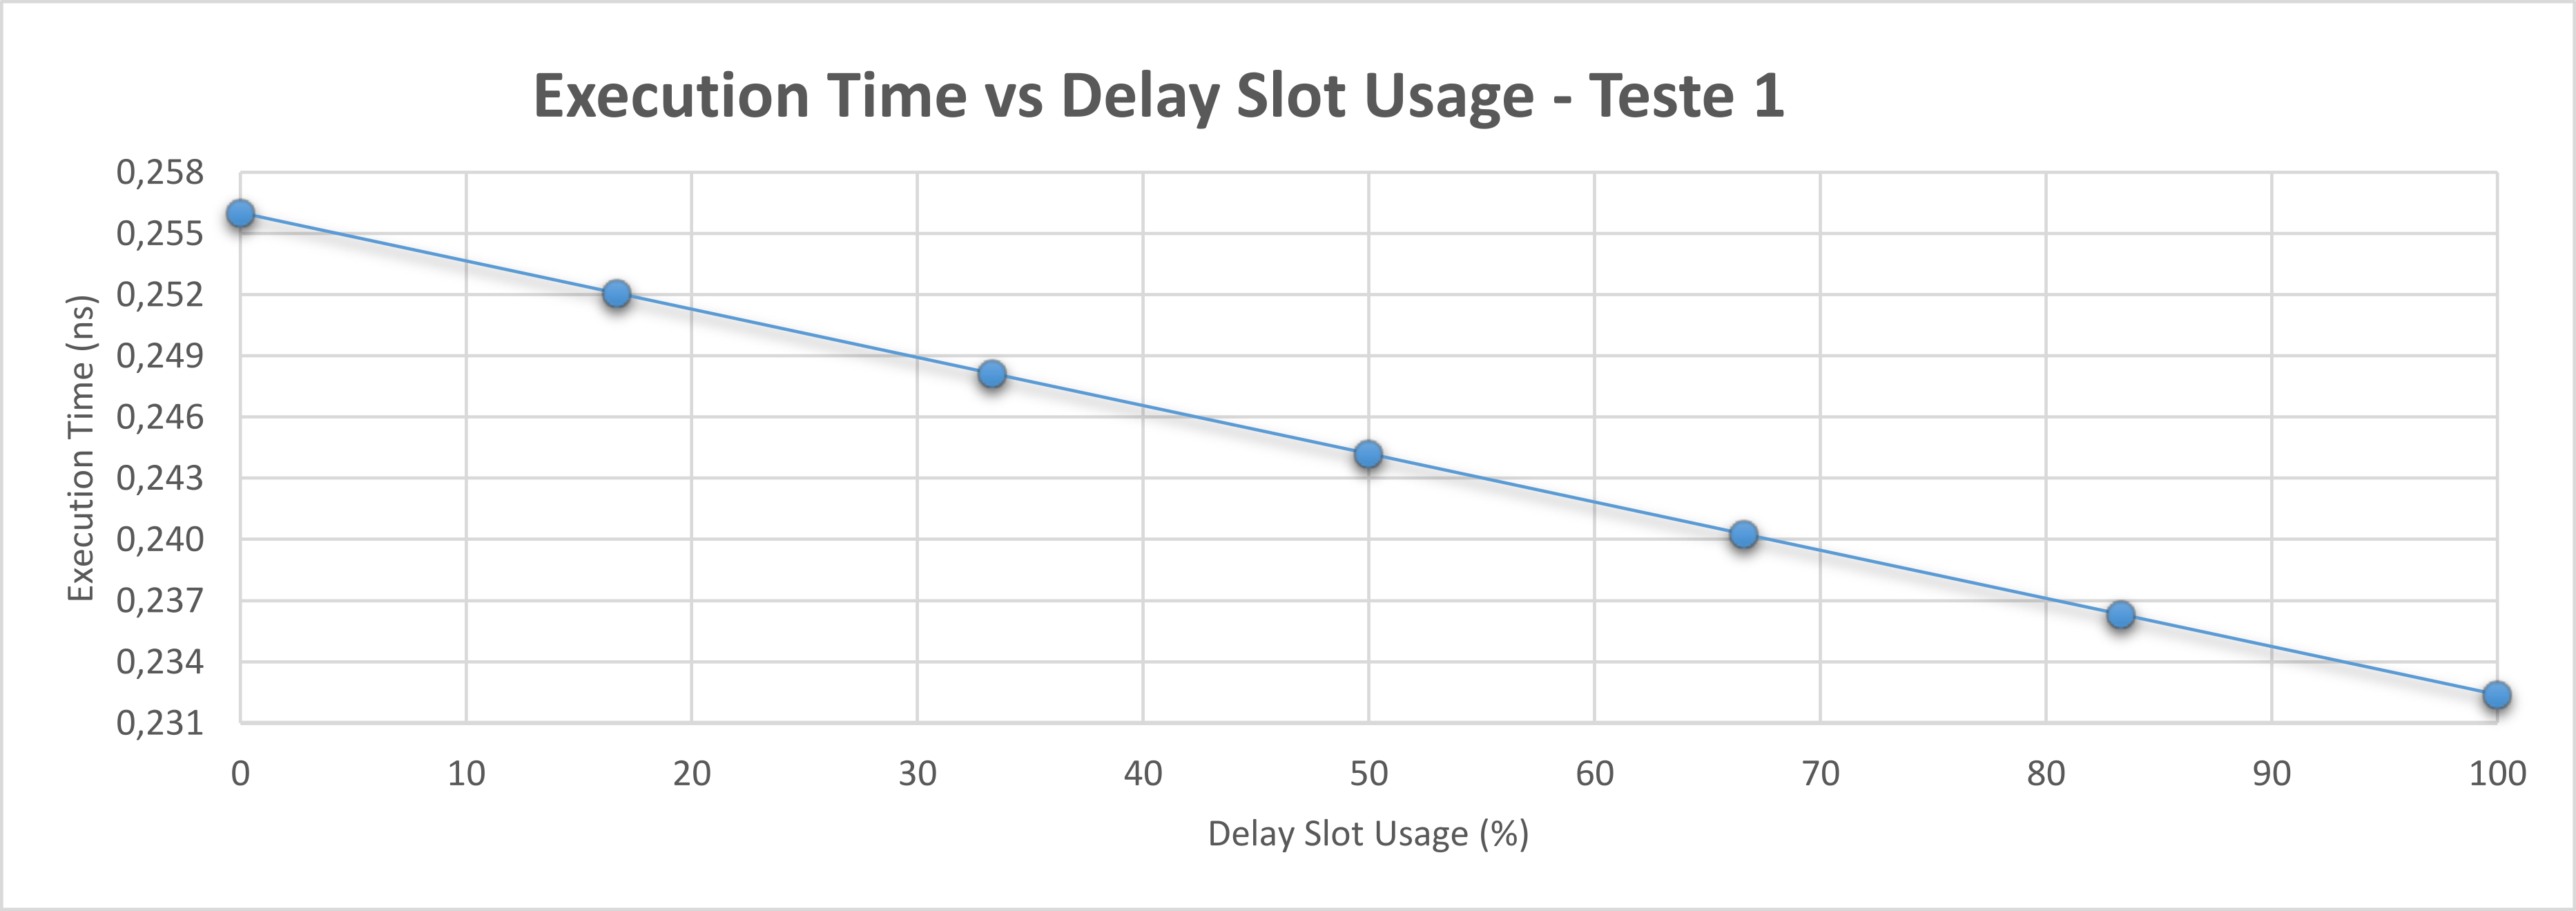
\includegraphics[clip, keepaspectratio=true, scale=1]{./images/teste1.png}}
		\caption{Relação Tempo de execução - Utilização do Delay Slot para Teste 1}
		\label{tempexet1}
	\end{center}
\end{figure}

\begin{figure}[H]
	\begin{center}
		\makebox[\textwidth][c]{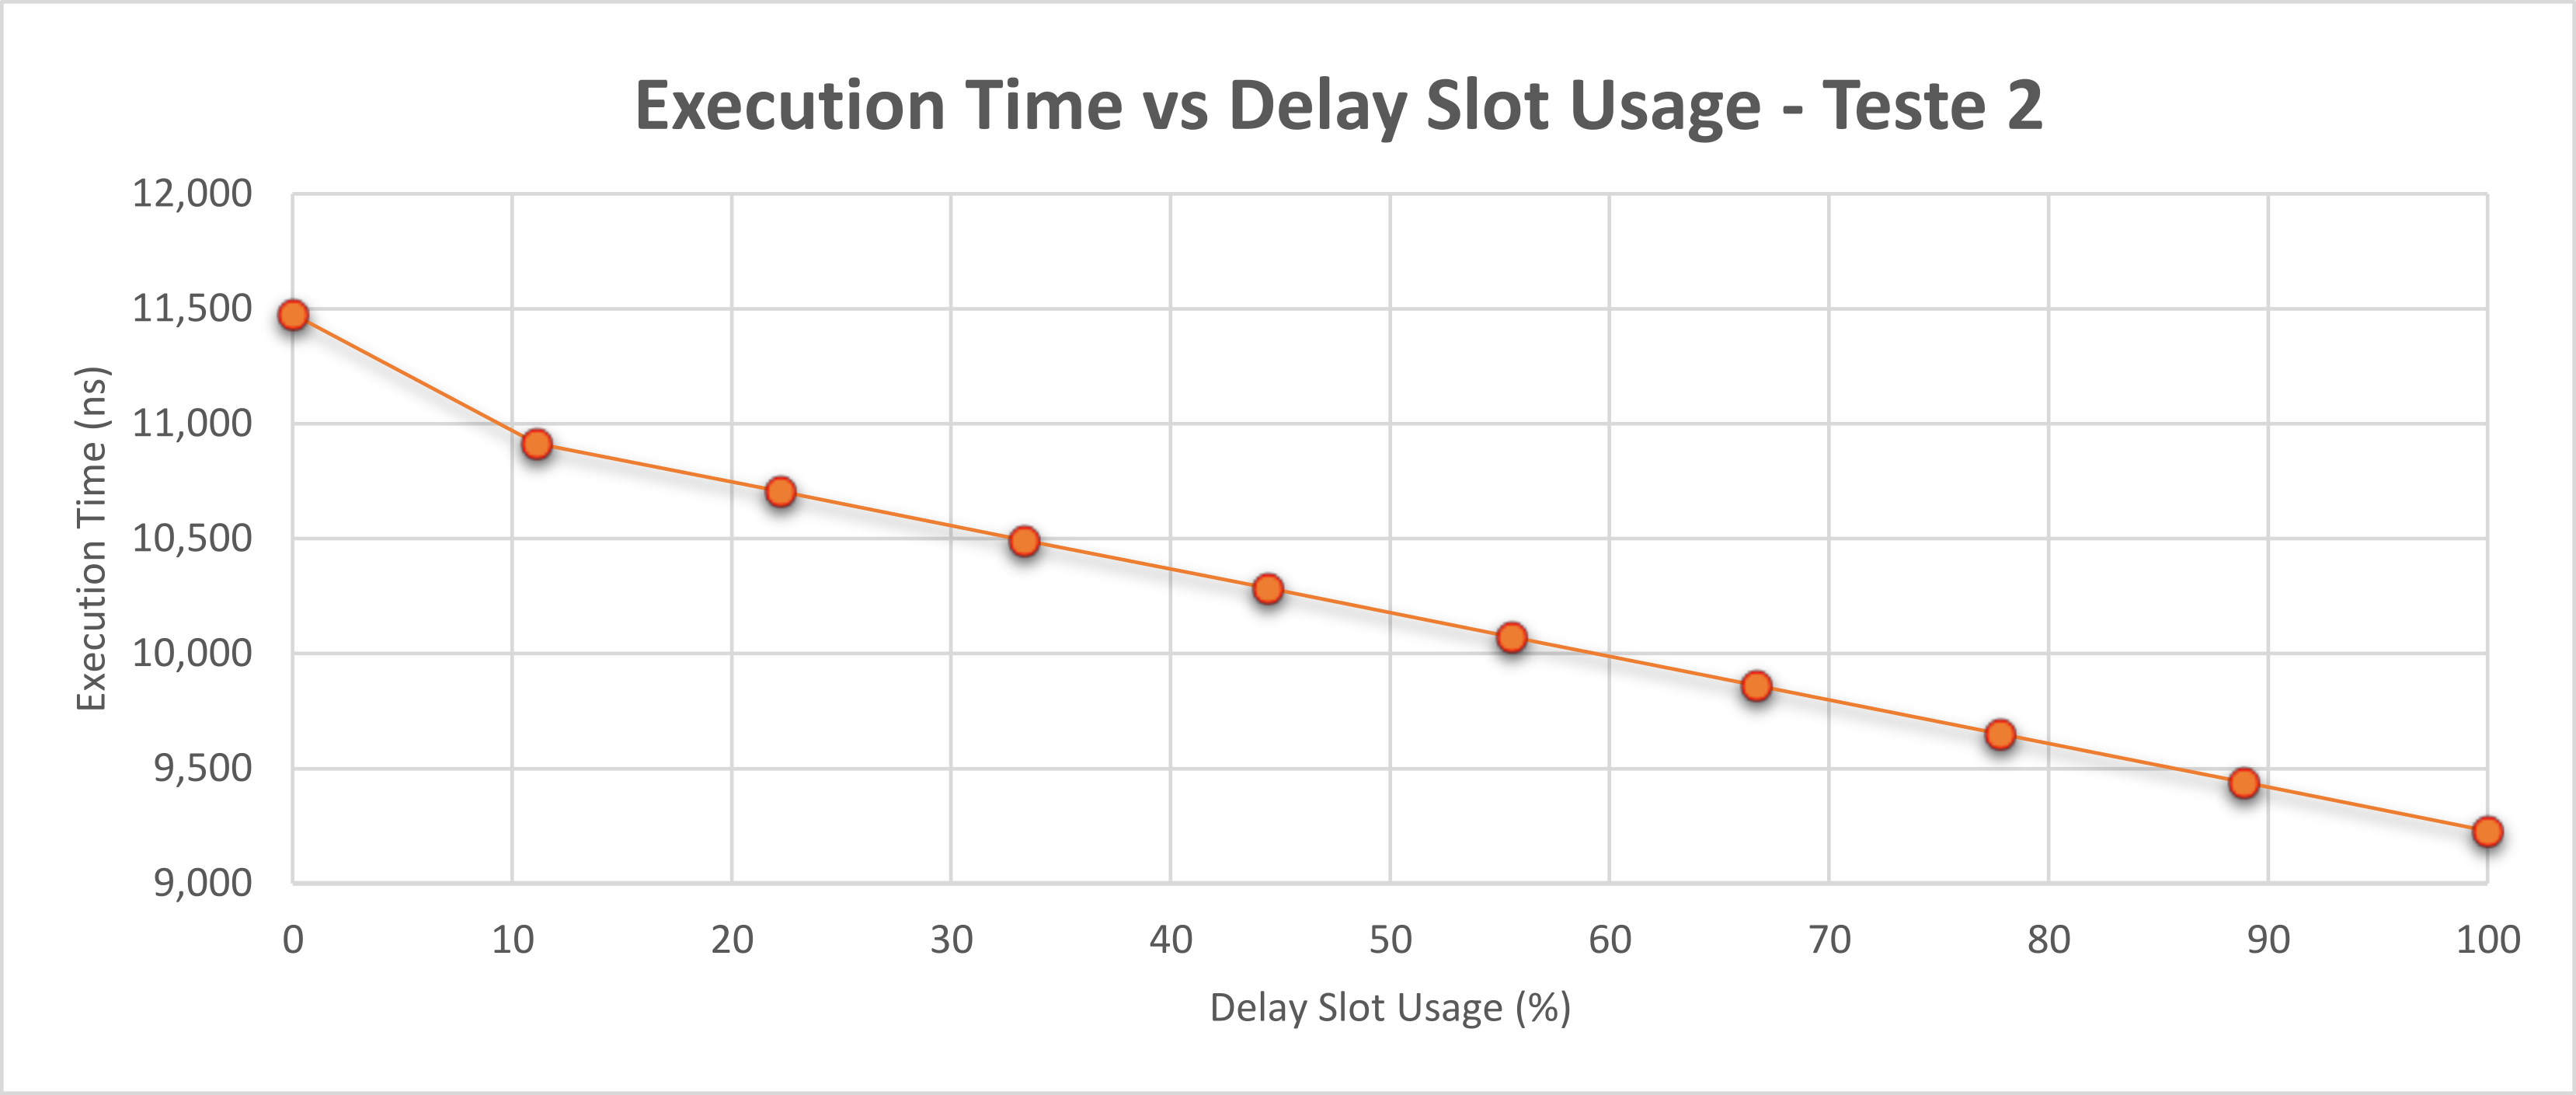
\includegraphics[clip, keepaspectratio=true, scale=1]{./images/teste2.png}}
		\caption{Relação Tempo de execução - Utilização do Delay Slot para Teste 2.}
		\label{tempexet2}
	\end{center}
\end{figure}

\begin{figure}[H]
	\begin{center}
		\makebox[\textwidth][c]{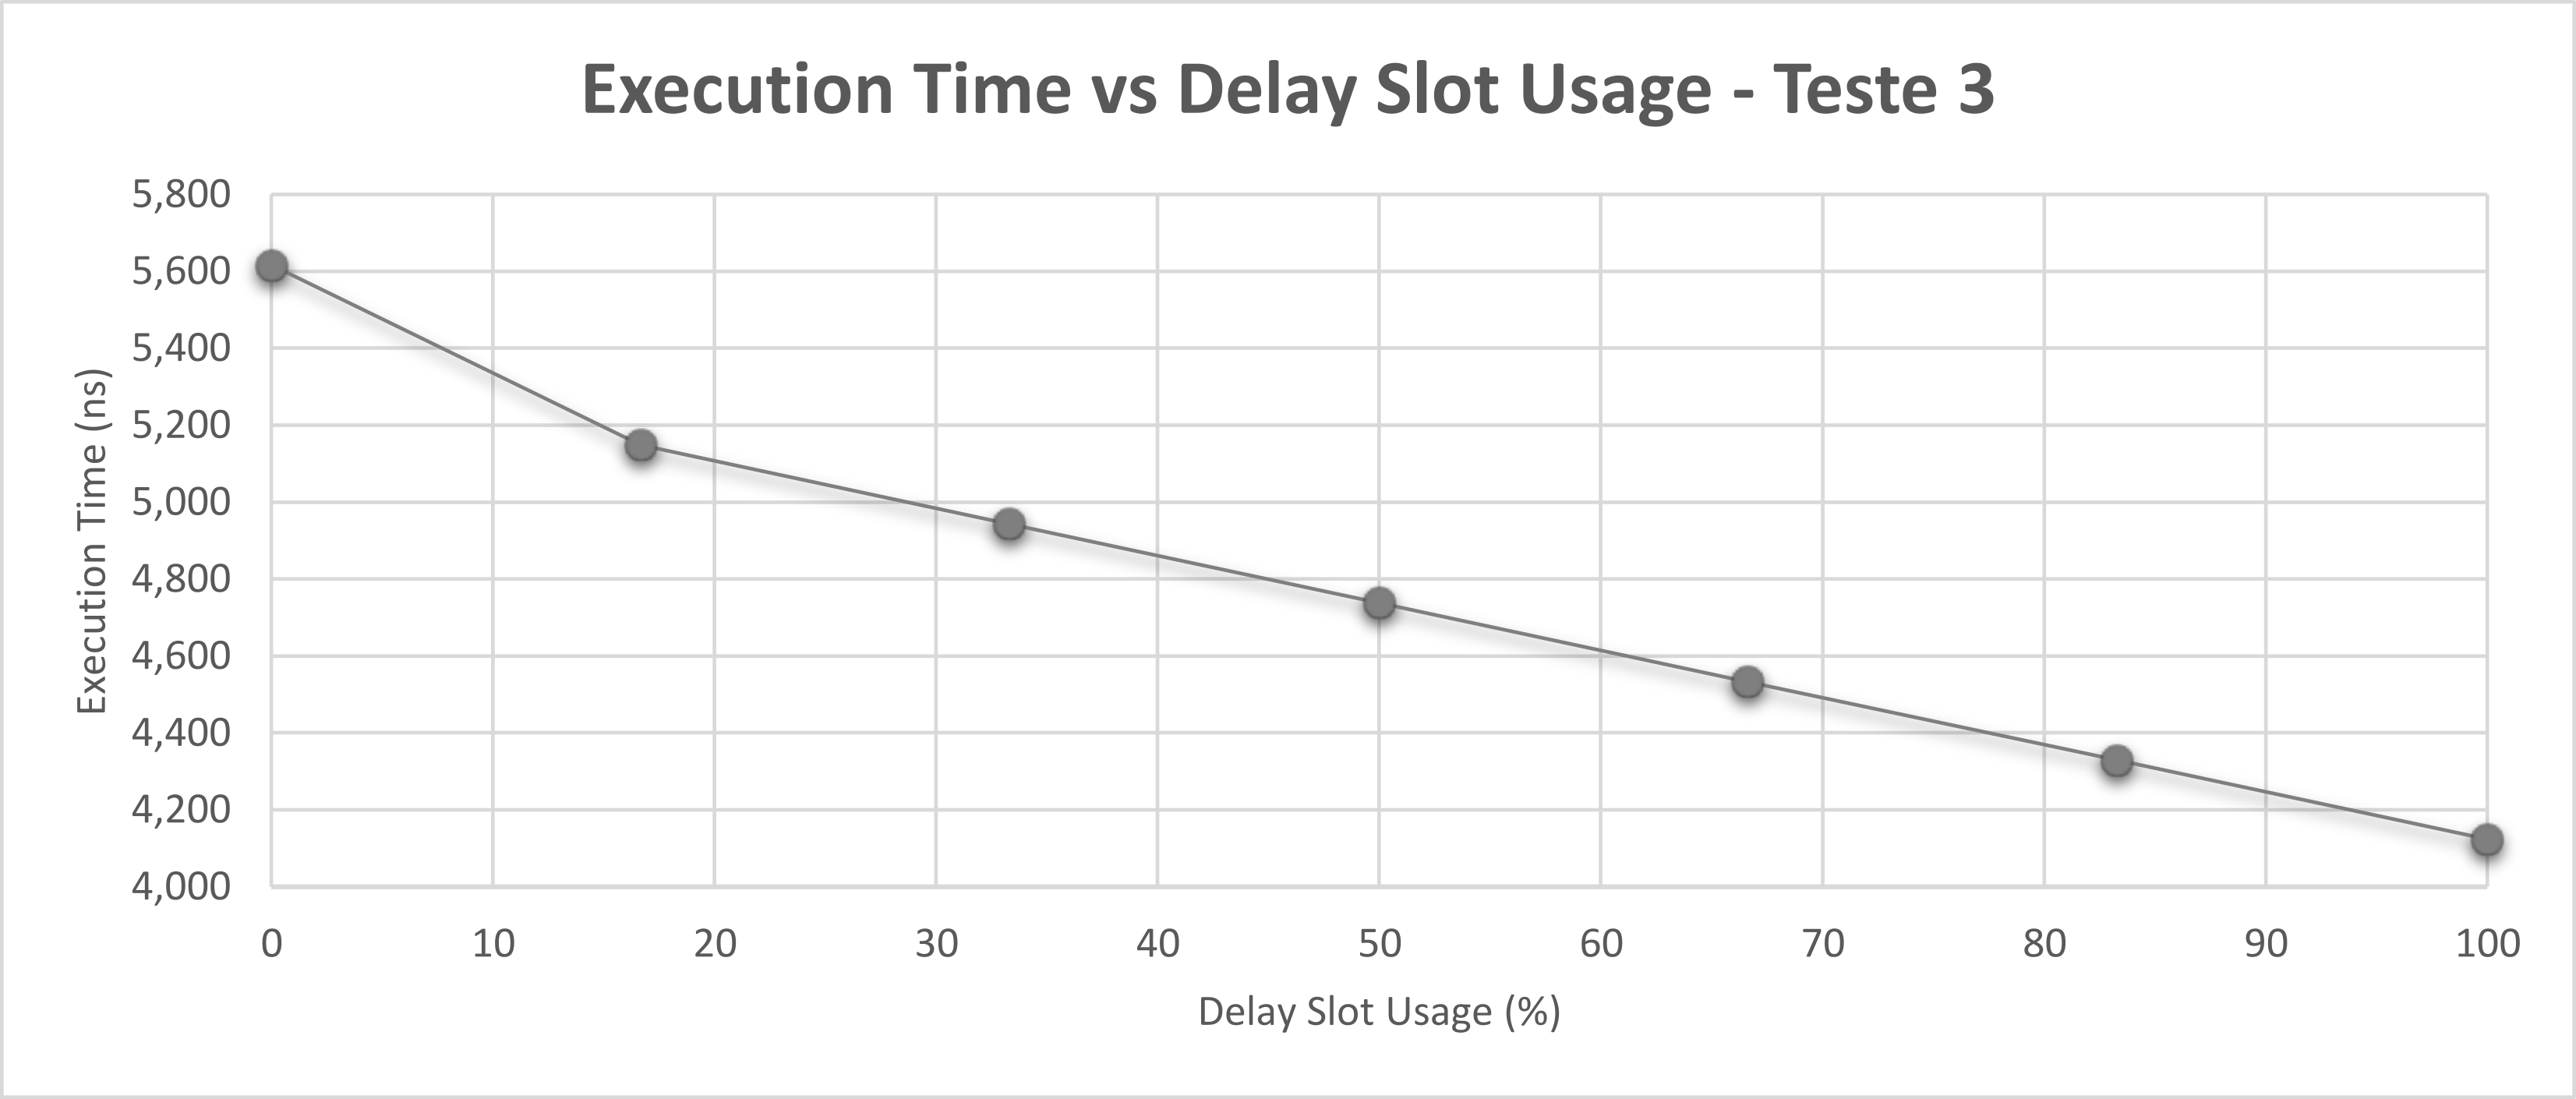
\includegraphics[clip, keepaspectratio=true, scale=1]{./images/teste3.png}}
		\caption{Relação Tempo de execução - Utilização do Delay Slot para Teste 3.}
		\label{tempexet3}
	\end{center}
\end{figure}

\begin{figure}[H]
	\begin{center}
		\makebox[\textwidth][c]{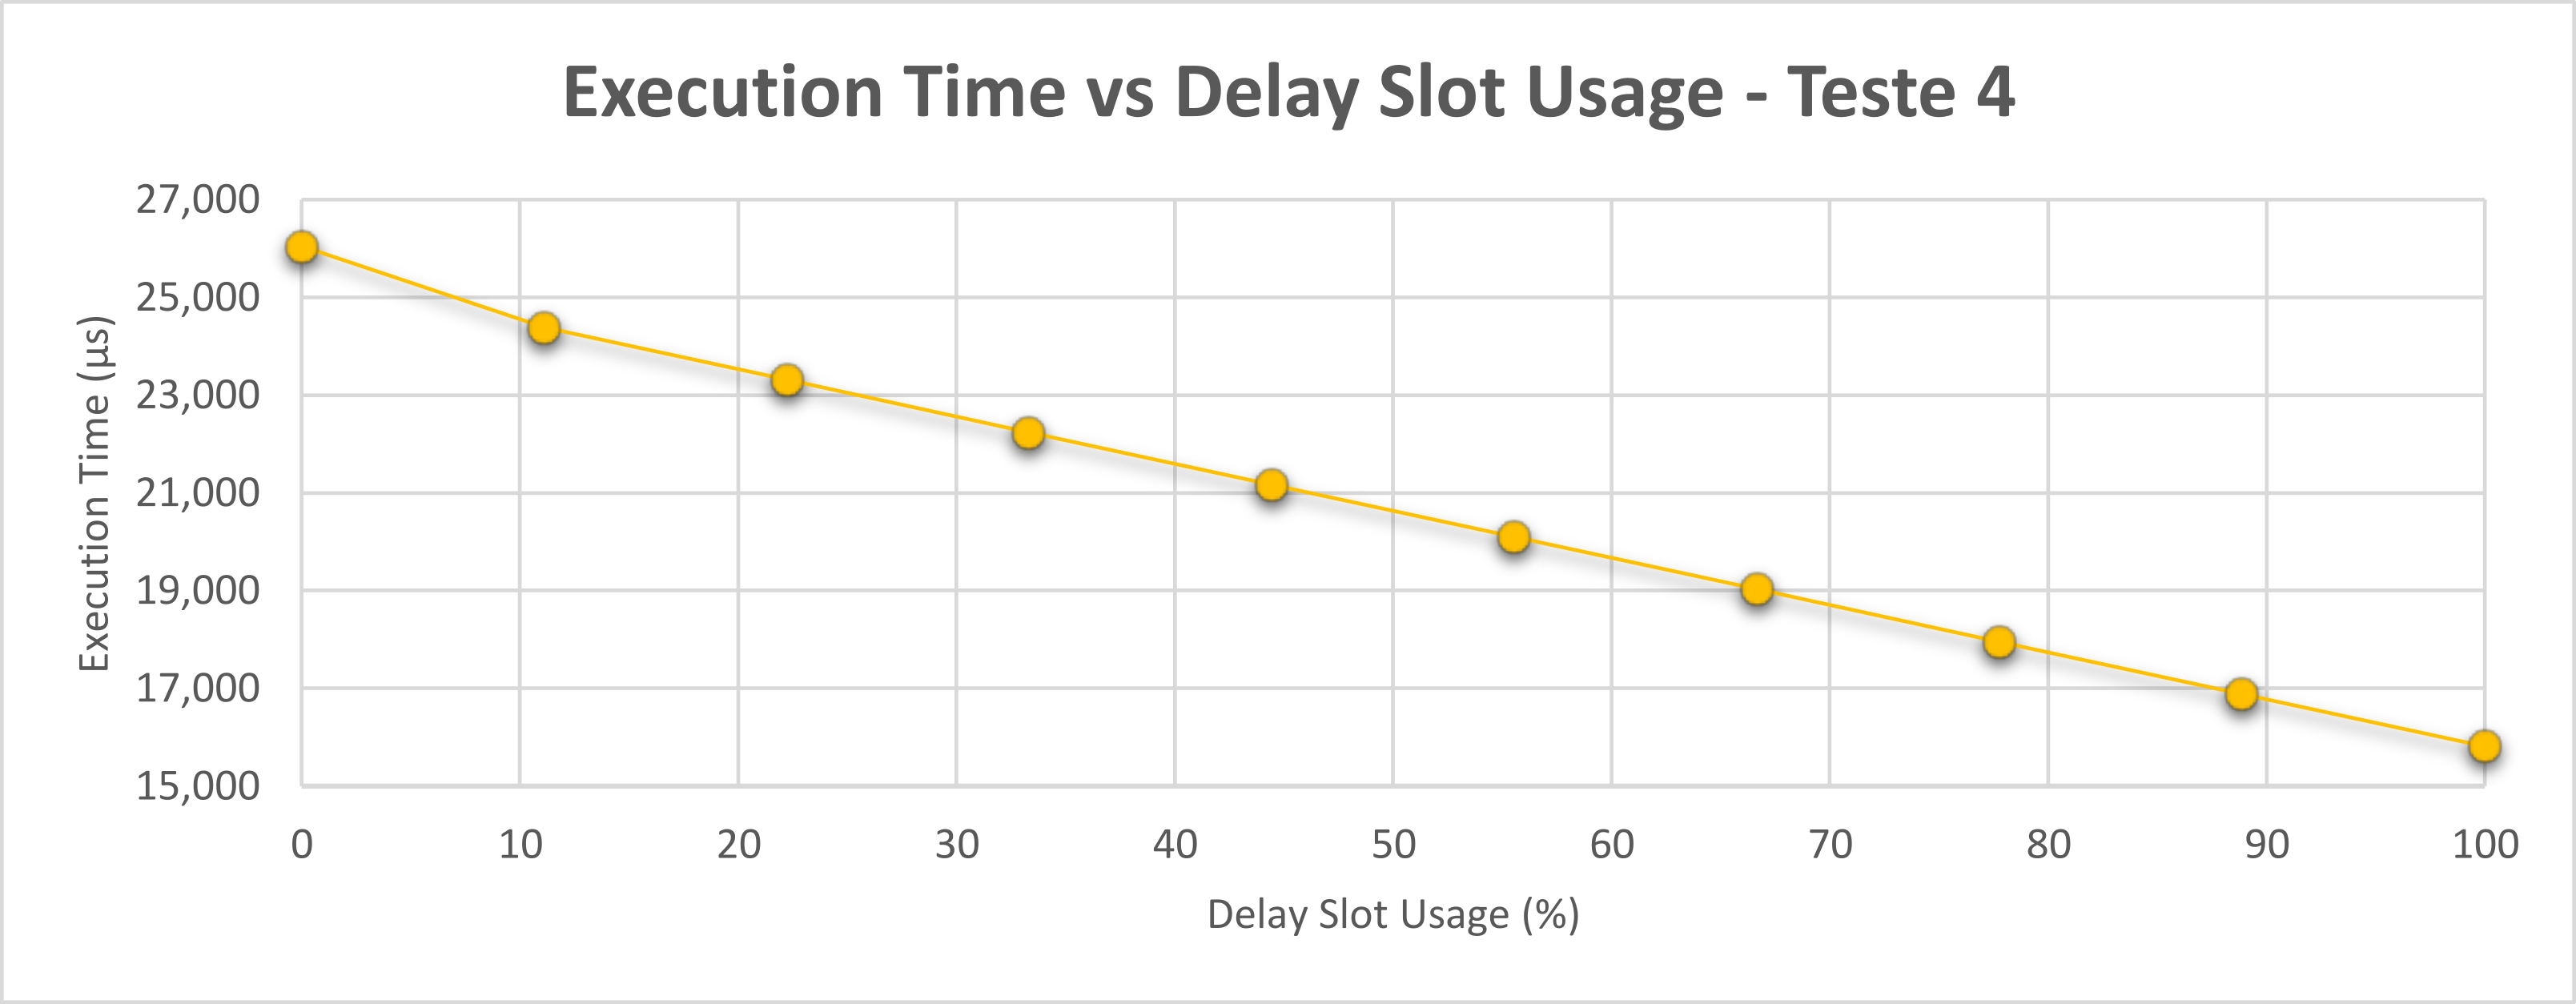
\includegraphics[clip, keepaspectratio=true, scale=1]{./images/teste4.png}}
		\caption{Relação Tempo de execução - Utilização do Delay Slot para Teste 4.}
		\label{tempexet3}
	\end{center}
\end{figure}